\chapter{Introduction to deep learning}
\section{Forward Propagation}
Let us build a neural network from scratch and code how it performs predictions using forward propagation. Please note that all deep learning libraries have the entire training and prediction processes implemented, and so in practice you wouldn't really need to build a neural network from scratch. However, this is still good to know to help understanding how they work.

\begin{figure}[htp]
	\centering
	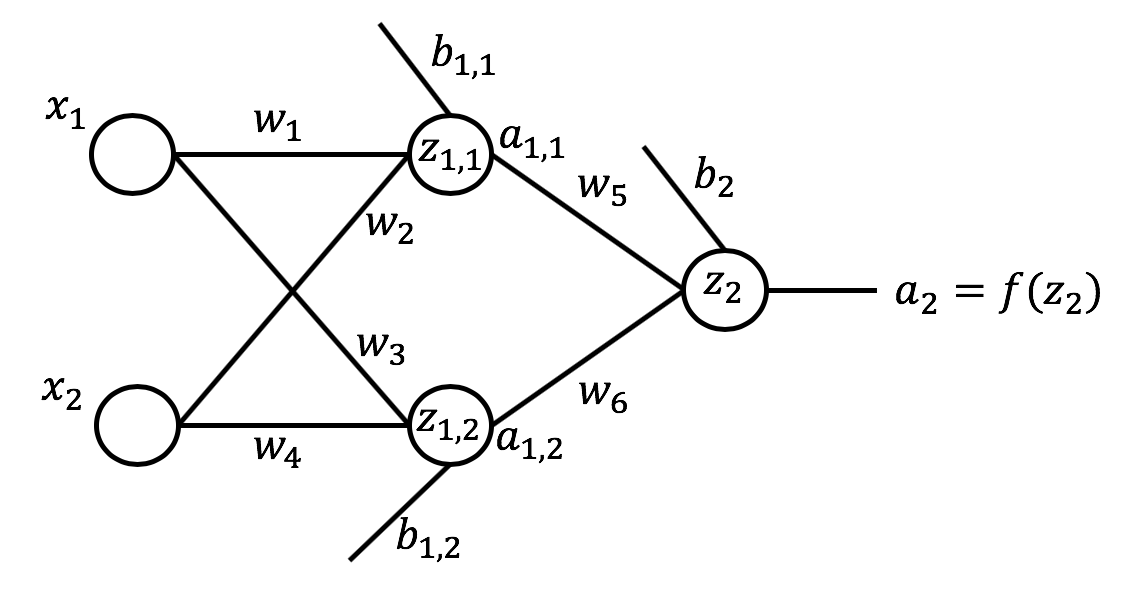
\includegraphics[width=\linewidth]{Assets/neural_network_example}
	\caption{A neural network that takes two inputs, has one hidden layer with two nodes, and an output layer with one node.}
	\label{fig:neural network}
\end{figure}

\noindent Let's start by randomly initializing the weights and the biases in the network. We have 6 weights and 3 biases, one for each node in the hidden layer as well as for each node in the output layer.

\noindent We would then calculate the weighted sum of the input at the hidden layer. It follows that:

\begin{equation} \label{weighted sum}
	\begin{split}
		z_{1,1} & = x_1 \cdot w_1 + x_2 \cdot w_2 + b_{1,1}\\
		z_{1,2} & = x_1 \cdot w_3 + x_2 \cdot w_4 + b_{1,2}
	\end{split}
\end{equation}

\noindent Next, assuming a sigmoid activation function, let's compute the activation of the nodes,  $a_{1,1}$ and $a_{1,2}$ , in the hidden layer.

\begin{equation} \label{activation nodes}
	\begin{split}
		a_{1,1} & = \frac{1}{1+e^{-z_{1,1}}}\\
		a_{1,2} & = \frac{1}{1+e^{-z_{1,2}}}
	\end{split}
\end{equation}

\noindent These activations would serve as inputs to the next hidden layer or in this case the output layer. Let us compute the weighted sum of these inputs to the node in the output layer.

\begin{equation} \label{output layer}
	\begin{split}
		z_2 & = a_{1,1} \cdot w_5 + a_{1,2} \cdot w_6 + b_2
	\end{split}
\end{equation}

\noindent Finally, let's compute the output of the network as the activation of the node in the output layer.

\begin{equation} \label{output nodes}
	\begin{split}
		a_2 & = \frac{1}{1+e^{-z_2}}\\
	\end{split}
\end{equation}

\noindent The activation of the node in the output layer which is equivalent to the prediction made by the network.